%!TEX root = main.tex

% =============================================================================
\section{Uncertainty Benchmark}
\label{sec:uncertainty-benchmark}
% =============================================================================

In this section, we describe an uncertainty benchmark that we use to evaluate
    the robust tuning configurations given by \Endure, both analytically using
    the cost models, and empirically using RocksDB.
It consists of two primary components: (1) \emph{Expected workloads} and,
    (2) \emph{Benchmark set of sampled workloads}, described below.

\Paragraph{Expected Workloads}
We create robust tunings configurations for 15 expected workloads encompassing
    different proportions of query types.
We catalog them into \emph{uniform}, \emph{unimodal}, \emph{bimodal}, and
    \emph{trimodal} categories based upon the dominant query types.
% 4 unimodal workloads contain 97\% queries belonging to a single query type.
% 6 bimodal workloads have two query types accounting for 49\% of queries each, while
%     another 4 trimodal workloads have 33\% queries belonging to three query types.
% Lastly, a single uniform workload contains 25\% queries belonging to each of the four
%     different query types.
A minimum 1\% of each query type is always included in every expected workload
    to ensure a finite KL-divergence.
Henceforth, we use $\workload_i$ to refer to the $i$-th expected 
    workload from Table~\ref{tab:expected-workloads}.
\begin{table}[h]
    \centering%\small
    \begin{tabular}{c cccc l}
    \toprule
    Index & \multicolumn{4}{c}{$(\emptylookup, \nonemptylookup, \range, \update)$} & Type \\
    \toprule
    0 & 25\% & 25\% & 25\% & 25\% & \textbf{Uniform} \\
    \midrule
    1 & 97\% & 1\% & 1\% & 1\% & \textbf{Unimodal}\\
    2 & 1\% & 97\% & 1\% & 1\% & \\
    3 & 1\% & 1\% & 97\% & 1\% & \\
    4 & 1\% & 1\% & 1\% & 97\% & \\
    \midrule
    5 & 49\% & 49\% & 1\% & 1\% & \textbf{Bimodal}\\
    6 & 49\% & 1\% & 49\% & 1\% & \\
    7 & 49\% & 1\% & 1\% & 49\% & \\
    8 & 1\% & 49\% & 49\% & 1\% & \\
    9 & 1\% & 49\% & 1\% & 49\% & \\
    10 & 1\% & 1\% & 49\% & 49\% & \\
    \midrule
    11 & 33\% & 33\% & 33\% & 1\% & \textbf{Trimodal}\\
    12 & 33\% & 33\% & 1\% & 33\% & \\
    13 & 33\% & 1\% & 33\% & 33\% & \\
    14 & 1\% & 33\% & 33\% & 33\% & \\
    \bottomrule
    \end{tabular}
    \caption{Expected workloads.}
    \label{tab:expected-workloads}	
\end{table}

%\subsection{Benchmark Set of Sampled Workloads}
\begin{figure}
    \centering
    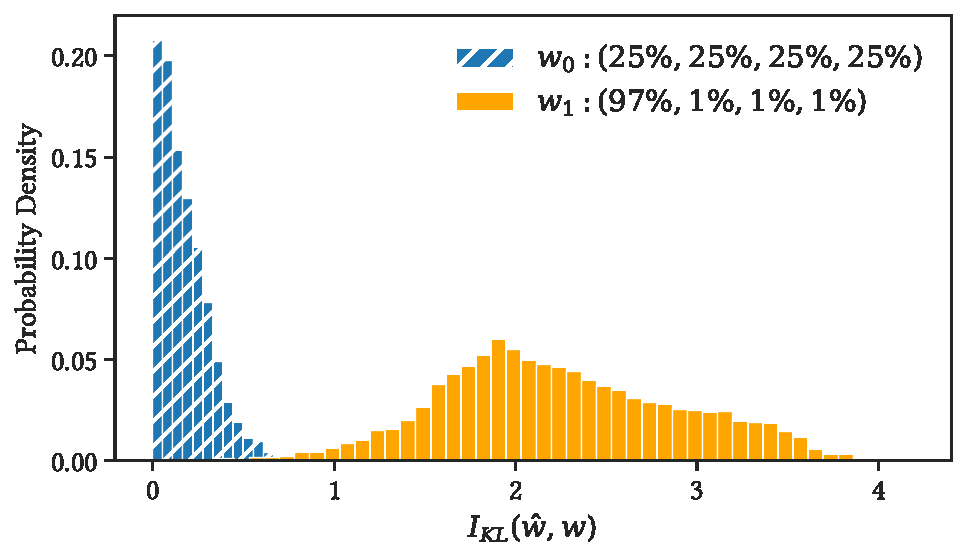
\includegraphics[scale=0.5]{figures/KL_divergence_histogram.pdf}
    \caption{KL-divergence $I_{KL}(\obsworkload, w)$ histograms of the sampled
        workloads wrt. to expected workloads $\workload_0$ and $\workload_1$.}
    \label{fig:KL_divergence_histogram}
\end{figure}

\Paragraph{Benchmark Set of Sampled Workloads}
We use the benchmark set of 10K workloads {\benchmark} as a \emph{test} dataset
    over which to evaluate the tuning configurations.
These configurations are generated as follows:
first, we independently sample the number of queries corresponding to each 
    query type uniformly at random from a range $(0, 10000)$ to obtain a $4$-tuple
    of query counts.
Next, we divide the individual query counts by the total number of queries in 
    the tuple to obtain a random workload that is added to the benchmark set.
We use the actual query counts during the system experimentation where we
    execute individual queries on the database.

Note that while the same {\benchmark}
    is used to evaluate different tunings, it represents a different 
    distribution of KL-divergences for the corresponding expected workload 
    associated with each tuning.
As an example, in Figure \ref{fig:KL_divergence_histogram}, we plot the 
    distribution of KL-divergences of sampled workloads in {\benchmark} 
    wrt. the expected workloads $\workload_0$ and $\workload_1$ from 
    Table \ref{tab:expected-workloads}.
